\section{Definitions and Numerical Computations of Lyapunov Exponents}

One of the key defining properties of chaos in dynamical systems is that small perturbations\footnote{A `small perturbation' of an initial point means to take a new point that is very close to the original.} in the initial conditions lead to large differences over time.
With the assumption that the distance of nearby points increases exponentially, the following simplistic formula for the dynamical system of an iterative map $F$ can be deduced
\begin{align}\label{eq:lyapunov_exponent}
    \left|F^n(x_0+\epsilon)-F^n(x_0)\right| \sim \epsilon e^{n \lambda}, \text{ as } n \rightarrow \infty,
\end{align}
where $\lambda$ is the \emph{Lyapunov exponent} \cite{nonlinear_system}\cite{lyapunov} and $x_0$ is the point at discrete time $0$.

A positive $\lambda$ means nearby points of $x_0$ will move away from it as time progresses, and a negative $\lambda$ means nearby points will converge to it. 
The absolute value of $\lambda$ represents the rate of divergence or convergence.

The existence of such $\lambda$ is not obvious, the analytical evaluation of $\lambda$ is often hopeless, and the assumption seems very questionable.
However, if acquiescing in such a formula, $\lambda$ can be calculated numerically, giving important insights into the dynamical system. 

Assuming that $\epsilon e^{n \lambda} \to 0$ and $\epsilon$ is small, \eqref{eq:lyapunov_exponent} becomes
$$
\epsilon \left| \frac{dF^n(x_0)}{dx} \right| \sim \epsilon e^{n \lambda} \text{ as } n \rightarrow \infty.
$$
Taking the logarithm,
\begin{align}
    \lambda 
    &= \lim_{n \to \infty}\left(\frac{1}{n}\ln{\left|\frac{dF^n(x_0)}{dx}\right|}\right)  \\
    &= \lim_{N \to \infty}\left\{\frac{1}{N}\sum_{n=0}^{N-1}\ln{|F'(x_n)|}\right\}  \label{eq:lambda},
\end{align}
where in the last step we labelled the points $x_1 = F(x_0), x_2 = F(x_1), \dots$ and applied the chain rule.
All of the numerical calculations of Lyapunov exponents in this report will use \eqref{eq:lambda}.

Equation \eqref{eq:lambda} fails to make sense at the points $x$ where $F'(x) = 0$.
Such points are called \emph{superstability} points, and the Lyapunov exponents of which are defined as $- \infty$.

The following are some examples of calculating Lyapunov exponents.

\begin{exmp}
	A classical example of chaotic system is generated by the iteration of the tent map, which is defined by
    \begin{align}
        F(r, x)= 
        \begin{cases}
            r x, & \text{ if } x \in [0,1/2) \\
            r (1-x), & \text{ if } x \in [1/2,1]
        \end{cases} \label{eq:tent}
    \end{align}
    where $r$ is a parameter.
	The Lyapunov exponent at $0$ is $\ln r$, which is negative if $r < 1$ and positive otherwise.
	The higher subfigure of Figure \ref{fig:lyapunov_tent} is the bifurcation diagram of the tent map, showing its dynamical properties. 
	It is obtained by selecting $1,000$ equally spaced $r \in [0,2]$, and for each $r$ picking a random starting point $x_0$, iterating $x_0$ for $10,000$ times, ignoring the first $1,000$ iterations, and plotting the rest of the $9,000$ $ x_i$ as a faint blue dot at coordinate $(r, x_i)$. 
	There is a dramatic change in behaviour exactly at $r=1$, where the Lyapunov exponent changed from negative to positive.
    For $r < 1$ every $x_0$ converged to $0$, whereas afterwards the system shows an apparent chaotic behaviour by casting an interesting homogeneous shape of a double curved triangle. At $r = 2$, this system can be proved to be chaotic as will be shown in Example \ref{ex:logistic and tent}.

    \begin{figure}
        \centering
        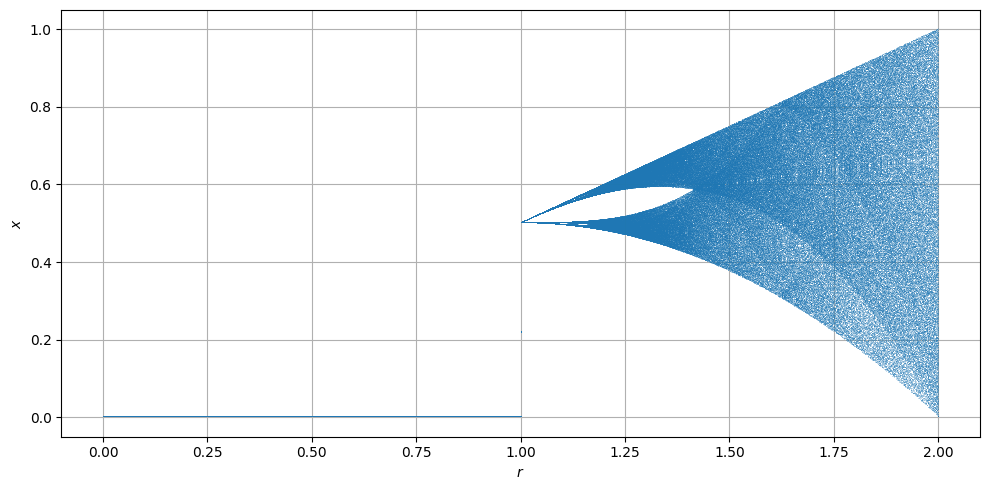
\includegraphics[width=\linewidth]{Bifurcation Images/bifurcation_tent.png}
        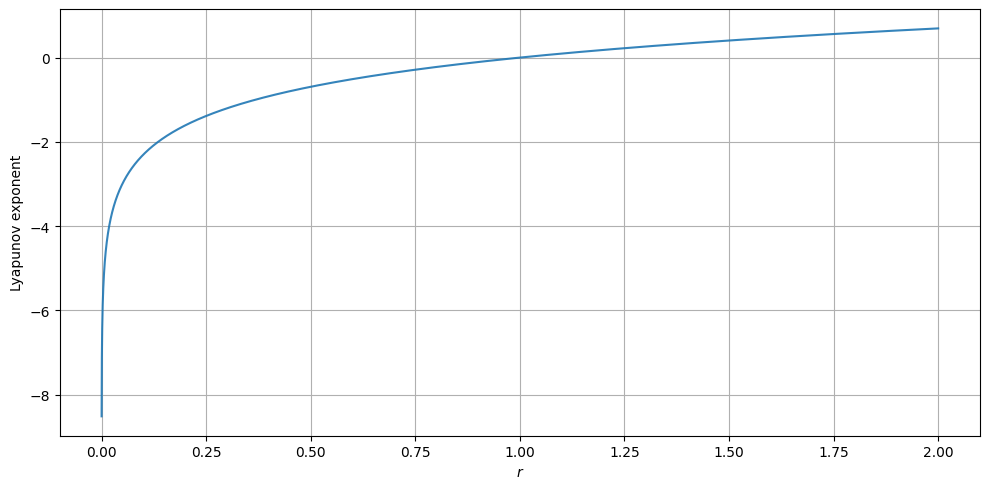
\includegraphics[width=\linewidth]{Bifurcation Images/lypaunov_tent.png}
        \caption{Bifurcation diagram (above) and Lyapunov exponent plot (below) for the tent map \eqref{eq:tent} over 10,000 iterations.}
        \label{fig:lyapunov_tent}
    \end{figure}
\end{exmp}

\begin{exmp}
	Similarly, consider the dynamical system depending on one parameter $r$ generated by the iterations of the map
    $F(r,x)=x^2+r$ where $x,r \in \mathbb{R}$.
	Unlike the case of the tent map, there is no simple closed form for the Lyapunov exponent, and computer simulations are required. 
	The bifurcation diagram and the Lyapunov exponent are shown in Figure \ref{fig:lyapunov_x^2}.
    \begin{figure}
        \centering
        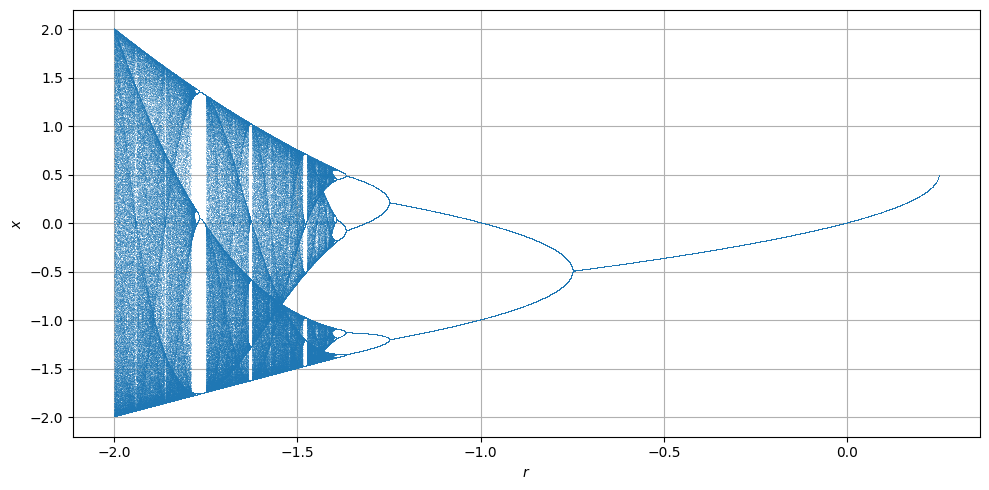
\includegraphics[width=1\linewidth]{Bifurcation Images/bifurcation_quadratic.png}
        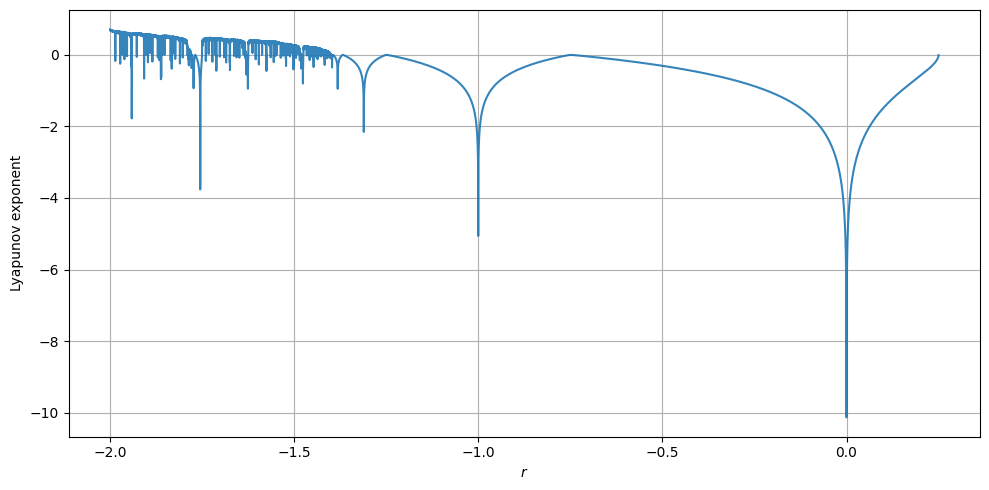
\includegraphics[width=1\linewidth]{Bifurcation Images/lypaunov_quadratic.png}
        \caption{Bifurcation diagram (above) and Lyapunov exponent plot (below) for the map $F(\lambda,x)=x^2+r$ over 50,000 iterations.}
        \label{fig:lyapunov_x^2}
    \end{figure}
	A very interesting phenomenon of periodic doubling is apparent from the bifurcation diagram (which is studied in detail in Chapter \ref{chapter:bifurcation}).
	Similar to the tent map, regions where the Lyapunov exponent is negative correspond to distinct lines in the bifurcation diagram, while those with a positive Lyapunov exponent correspond to chaotic bands.
\end{exmp}


\section{Lyapunov Exponents for a Continuous Time Series}\label{LyapCts}

The Lyapunov exponents for continuous time dynamical systems in multiple dimensions exhibit very different behaviours compared to the simplistic one dimensional discrete time dynamical systems discussed in the previous section. 
For continuous systems, we need to consider the complete spectrum of Lyapunov exponents. 
Given a continuous dynamical system in an $n$-dimensional phase space, we monitor the long-term evolution of an infinitely small $n$-sphere of initial conditions. 
It quantifies the average exponential growth or decay rates of perturbations in different directions in phase space. 
For an $n$-dimensional system, the Lyapunov spectrum consists of $n$ exponents, $\lambda_1 \geq \lambda_2 \geq \dots \geq \lambda_n$, which describe the system's behaviour in terms of expanding, neutral, and contracting directions. We can compute the spectra numerically.

Let's consider a continuous-time dynamical system defined by
$$
\dot{\mathbf{x}}(t) = \mathbf{f}(\mathbf{x}(t)),
$$
where $\mathbf{x}(t) \in \mathbb{R}^n$ is the state vector, and $\mathbf{f}$ is a smooth vector field and $t \geq0$ with initial conditions of $\mathbf{x}(0)=\mathbf{x_0}$. As with discrete systems, we may analyse the effects of initial perturbations on trajectories to determine whether they expand or contract. By using the trajectory $\mathbf{x}(t)$ and some nearby perturbation $\mathbf{y}=\delta\mathbf{x}(t)$, the linearised system becomes
$$
\dot{\mathbf{y}}(t) = \mathbf{J}(\mathbf{x}(t))\mathbf{y}(t),
$$
where $\mathbf{J}(\mathbf{x}(t))$ is the Jacobian matrix of $\mathbf{f}$ evaluated at $\mathbf{x}(t)$
$$
\mathbf{J}(\mathbf{x}(t)) = \frac{\partial \mathbf{f}}{\partial \mathbf{x}} \bigg|_{\mathbf{x}(t)}.
$$
The solution at the initial perturbation $\mathbf{y}(0)$ can be shown as $\mathbf{y}(t)=\mathbf{Y}(t)\mathbf{y}(0)$ where $\mathbf{Y}(t)$ is the fundamental solution, which satisfies
$$
\dot{\mathbf{Y}}=\mathbf{J}(\mathbf{x}(t))\mathbf{Y},
$$
where $\mathbf{Y}(0)$ is the identity matrix. Assume that $\det \mathbf{Y}(t)>0$, such that the initial perturbed trajectories never meet. The fundamental solution can be visually interpreted as an $n$-dimensional sphere of initial conditions evolving into an $n$-dimensional ellipsoid due to the locally deforming nature of the trajectories. The principal axis of the ellipsoid determines the Lyapunov vectors that grow or shrink at rates determined by the Lyapunov exponents. The principal axis are the directions along which the ellipsoid stretches or contracts the most where the Lyapunov vectors are the time-dependent vectors that align with the directions of the principal axis. Each Lyapunov vector $\mathbf{p}_i(t)$ stretches or contracts at a rate given by their corresponding Lyapunov exponent $\lambda_i$. The Lyapunov vectors are given as
$$
\mathbf{p}_i(t)=\mathbf{Y}(t)\xi_i(t),
$$
where $\xi_i(t)$ are the eigenvectors of $\sqrt{\mathbf{Y}^T\mathbf{Y}}$. Since the Lyapunov exponent measures the distance in the rate of growth or decay between the perturbations, we need to compute the length of the Lyapunov vector. Thus we take the norm of the principal axis. Using the same logic as for a discrete system, the $i$th Lyapunov exponent \cite{OED} is 
\begin{align}
    \lambda_i=\lim_{t \to \infty}\frac{1}{t}\ln ||\mathbf{p}_i(t)||.  \label{eq:lyapunov_cont} 
\end{align}

The Lyapunov exponents describe the long-term average exponential growth rates of perturbations in different directions or the $i$-th principal axis of the ellipsoid. A positive exponent ($\lambda_i > 0$) indicates expansion in the corresponding direction. A zero exponent ($\lambda_i = 0$) indicates a neutral direction, such as along the flow of a trajectory. A negative exponent ($\lambda_i < 0$) indicates contraction in the corresponding direction.

Note that we can also solve for the $i$-th Lyapunov exponent $\lambda_i$ using $\log_2,$
\begin{align}
    \lambda_i = \lim_{t \to \infty} \frac{1}{t} \log_2 ||\mathbf{p}_i(t)||, \label{eq:continuous}
\end{align}
in order to show that the ellipsoid grows with a rate of $2^{\lambda_1t}$. The area of the ellipsoid is defined by the first two principal axes $2^{(\lambda_1+\lambda_2)t}$, the volume by the first three, $2^{(\lambda_1+\lambda_2+\lambda_3)t},$ and so on. \cite{continuouslyapunov}

For dissipative systems (systems that release energy instead of retaining it), the sum of the Lyapunov exponents is negative, indicating that the volume of the ellipsoid contracts over time.

In three dimensions, the sum of all the Lyapunov exponents is equivalent to the trace of the system's corresponding Jacobian matrix. 
In order for the system to be chaotic, only one of the individual exponents needs to be positive.
The possible Lyapunov spectra and the corresponding attractors are: $(+,0,-)$, which signifies chaotic behaviour; $(0,0,-)$, which tells us that the system will demonstrate quasi-periodic behaviour;
$(0,-,-)$, which corresponds to the presence of a limit cycle or periodic behaviour; and $(-,-,-)$ , which tells us that there is a stable fixed point. 
The sum of the Lyapunov exponents equals the time-averaged divergence of the phase space velocity. 
The value indicates the divergence of the flow and is the fractional rate of the volume expansion or contraction of the system, but for a conservative or Hamiltonian system, this sum is zero. 
For dissipative systems, this sum is negative, ensuring that at least one exponent is negative. 
As a result, the long-term motion of trajectories converge to a limit set with zero volume, known as an attractor. 
While Lyapunov exponents are defined based on long-time averages, short trajectories may not fully capture the distinct behaviours associated with positive, zero, and negative exponents. \cite{continuouslyapunov}

% To compute the Lyapunov spectrum numerically, we start by linearising the system by solving for the Jacobian matrix $\mathbf{J}(\mathbf{x}(t))$ along the reference trajectory $\mathbf{x}(t)$. We then need to evolve the perturbation vectors. We need to initialize a set of $n$ orthonormal perturbation vectors $\{\mathbf{v}_1, \mathbf{v}_2, \dots, \mathbf{v}_n\}$ and evolve them using the linearised dynamics
% $$
% \dot{\mathbf{v}}_i(t) = \mathbf{J}(\mathbf{x}(t)) \mathbf{v}_i(t).
% $$
% Subsequently we need to use the Gram Schmidt reorthonormnalisation on the vector frame that we created in order to to maintain their independence and prevent numerical overflow. Then we can track the growth rates of the perturbation vectors and accumulate their logarithmic growth rates
% $$
% \sum_{i=1}^n \ln \|\mathbf{v}_i(t)\|.
% $$
% where the Lyapunov exponents are computed as the time-averaged logarithmic growth rates
% $$
% L_i = \lim_{t \to \infty} \frac{1}{t} \ln\frac{\|\mathbf{v}_i(t)\|}{\|\mathbf{v}_i(0)\|}.
% $$


\begin{exmp} An example of a continuous dynamical system is the Lorenz system \ref{lorenzequation} using the parameter values of $ \sigma = 10, \rho = 28 $ and $ \beta = 8/3$. Solving for the system's Jacobian allows for the use of $QR$ decomposition on the corresponding eigenvectors. After substituting the norm of these vectors and re-orthonormalising them, we can then obtain their average as we vary the time. \cite{OED}
\begin{figure}
    \centering
    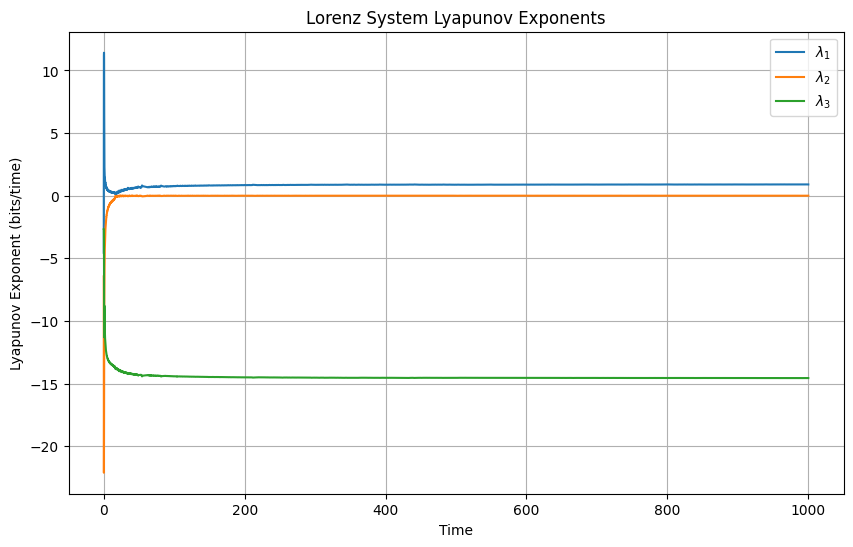
\includegraphics[width=1\linewidth]{Images/lorenz_lypunov.png}
    \caption{All values of $\lambda_i$ iterated over varying increasing time for the Lorenz system with parameter values of $\sigma = 10, \rho = 28$ and $\beta = 8/3$ with initial position of $(x,y,z)=(0.1,0.1,0.1)$. One exponent, $\lambda_1$ is shown to be greater than zero implying that at the conditions the system experiences chaos.}
    \label{fig:enter-label}
\end{figure}
As we iterate further in time, we get more accurate values for the different Lyapunov exponents, %$\lambda_i$
\begin{align*}
    \lambda_1 = 0.8973919196967531, \\
    \lambda_2 = 0.0000295072803878 ,\\
    \lambda_3 = -14.56408778526921,
\end{align*}
where $\lambda_1>0$, being positive, is responsible for the chaotic nature of the Lorenz system.
%which corresponds to the chaotic nature of the Lorenz system due to $\lambda_1>0$.
\end{exmp}
The first crucial step of this report is now complete; we have identified the key property of dynamical systems that attributes to chaos. We may now begin to investigate quantifiable properties of chaotic dynamical systems; the Lyapunov exponent will reappear throughout this task due to its importance.
% Given a continuous dynamical system in an $n$-dimensional phase space, we monitor the long-term evolution of an infinitesimal $n$-sphere of initial conditions. The sphere will become an $n$-ellipsoid due to the locally deforming nature of the flow. The $i$th one-dimensional Lyapunov exponent is then defined in terms of the length of the ellipsoidal principal axis $p_i(t)$
% \begin{align}
%     L_i=\lim_{n \to \infty} \frac{1}{n}\log_2\frac{p_i(t)}{p_i(0)} \label{eq:continous}
% \end{align}
% where $L_i$ are the individual exponents. Thus the Lyapunov exponents are related to the expanding or contracting nature of different directions in phase space. Since the orientation of the ellipsoid changes continuously as it evolves, the directions associated with a given exponent vary in a complicated way through the attractor. One cannot, therefore, speak of a well-defined direction associated with a given exponent. From \eqref{eq:continous} we can see that the ellipsoid grows with a rate of $2^{L_1t}$. The area is defined by the first 2 principle axis $2^{(L_1+L_2)t}$, and the volume by the third$2^{(L_1+L_2+L_3)t}$. From this we can create a new definition for the spectrum of exponents, the sum of the first $j$ exponents is define by the long term exponential growth rate of a $j$-volume element. This will provide us with a basis for the spectra technique fro experimental data.

% Any continuous time dependent dynamicla system without a fixed point will have at least one zero exponent which links with the slowly changing magnitude of a principle axis  tangent to the flow

% In a three-dimensional continuous dissipative dynamical system the only possible spectra, and the attractors they describe, are as follows: $( + , 0 , - )$ , a strange attractor; $(0,0,-)$, a two-toms; $(0, - , -)$, a limit cycle; and $( - , - , - )$ , The sum of each individual exponents is the time-averaged divergence of the phase space velocity; hence any dissipative dynamical system will have at least one negative exponent, the sum of all of the exponents is negative, and the post transient motion of trajectories will occur on a zero volume limit set, an attractor. Since Lyapunov exponents involve long-time averaged behavior, the short segments of the trajectories shown in the figure cannot be expected to accurately characterize the positive, zero, and negative exponents; nevertheless, the three distinct types of behavior are clear.

% The Lyapunov spectrum is closely related to the fractional dimension of the associated strange attractor.
%--------------------------------------------------------------------------------------------------%

% \textbf{Show that the $p$-cycle $\{X_1, X_2, \dots, X_p\}$ of the continuously differentiable map $F: \mathbb{R} \to \mathbb{R}$ is stable if  
% \[
% | F'(X_1) F'(X_2) \dots F'(X_p)| < 1.
% \]
% This is a proof the textbook refers to a lot in the section and I dont know how to interpret it or include it.}


% Idea: If we have an initial condition $x_0$ which will generate our sequence for a distcete dynamical system to use discrete time, and a point nearby $x_0 + \epsilon_0$. Let $\epsilon_n$= separation of orbits from $x_0$ and orbit from $x_0 + \epsilon_0$

% If $|\epsilon_n| \sim |\epsilon_0|e^{n\lambda}$ is converging exponentially, $\lambda$ is they lyanopunov exponent
% -$\lambda>0$ means chaos